\chapter{Basic data exploration}
\label{ch:basic_data_exploration}

\newthought{Let us consider another problem}, this time from clinical me\-di\-cine. We will dig for something interesting in the data and explore it with visualization widgets. You will get to know \mutation\ better, and also learn about several interesting visualizations.

We will start with an empty canvas; to clean it from our previous lesson, use either File/New or select all the widgets and remove them (use the backspace/delete key).

Now again, add the File widget and open another documentation data set: heart\_disease. How does the data look like?

\begin{figure}[h]
  \centering
  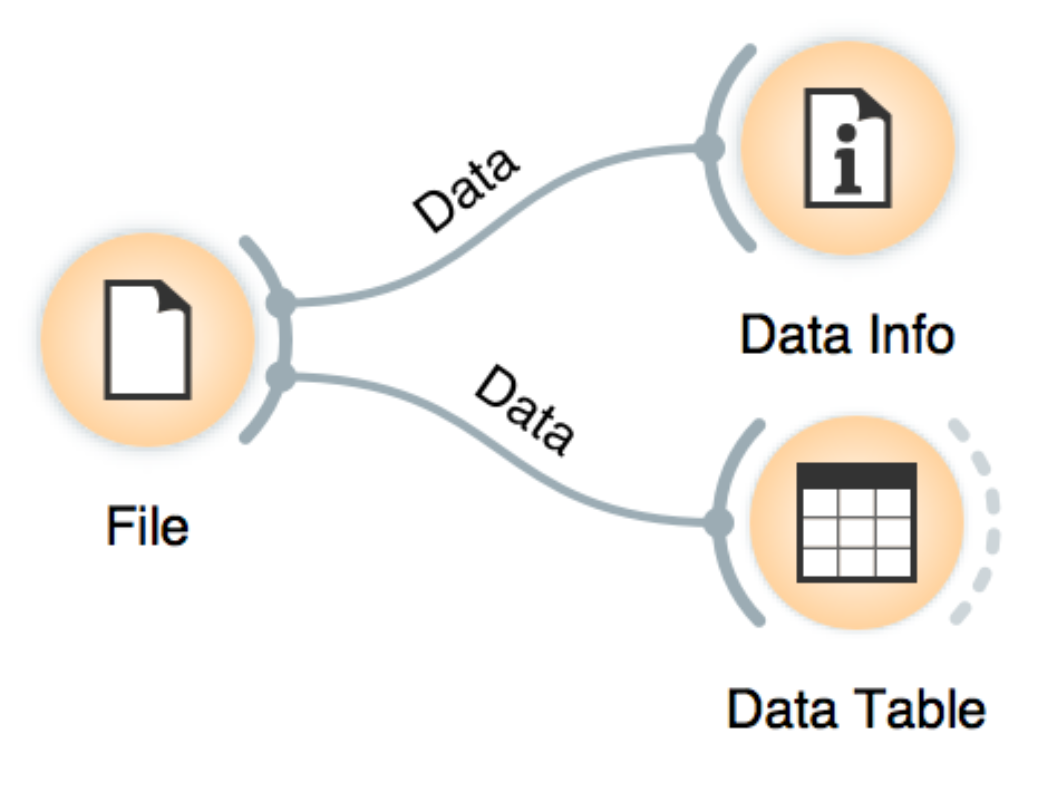
\includegraphics[width=50mm]{basic_data_exploration-fig1.png}%
  \caption{\textbf{\textsf{A simple workflow to inspect the loaded dataset.}}}
  \label{fig:basic_data_exploration-fig1}
\end{figure}

Let us check whether common visualizations tell us anything interesting. (Hint: look for gender differences. These are always interesting and occasionally even real.)

\begin{figure}[h]
  \centering
  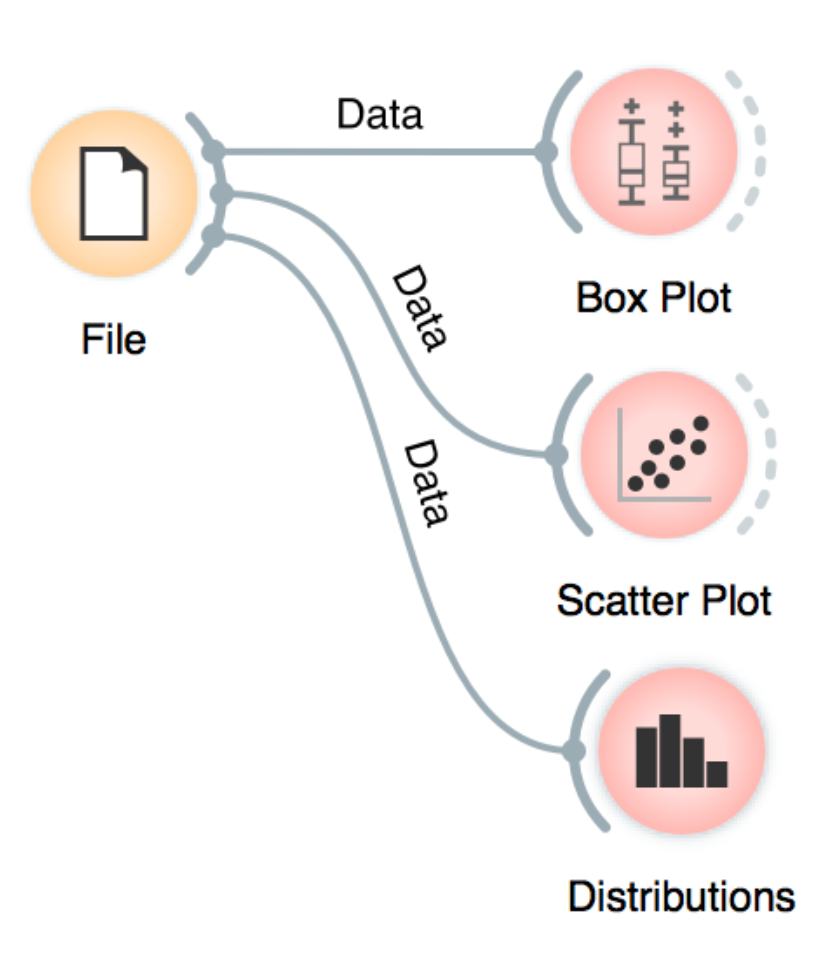
\includegraphics[width=50mm]{basic_data_exploration-fig2.png}%
  \caption{\textbf{\textsf{Quick check with common statistics and visualization widgets.}}}
  \label{fig:basic_data_exploration-fig2}
\end{figure}

\newpage
Data can also be split by the value of features, in this case the gender.

\begin{figure}[h]
  \centering
  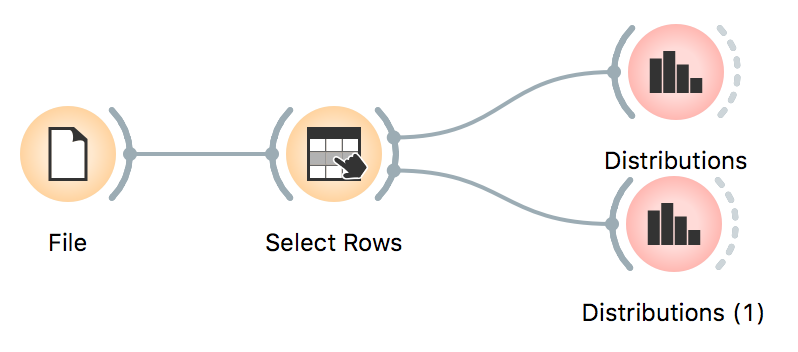
\includegraphics[width=90mm]{select-rows-workflow.png}%
  \caption{\textbf{\textsf{The two Distributions widgets get different data: the upper gets the selected rows and the lower gets the rest. Double-click the connection between the widgets to access setup dialog, as you've learned in the previous lesson.}}}
  \label{fig:basic_data_exploration-fig3}
\end{figure}

In the \widget{Select Rows} widget, we select the female patients. You can also add other conditions. The selection of data instances provides a powerful combination with visualization of data distribution. Try having at least two widgets open simultaneously and explore the data.

\begin{figure*}[h]
  \centering
  \newcommand{\selrow}{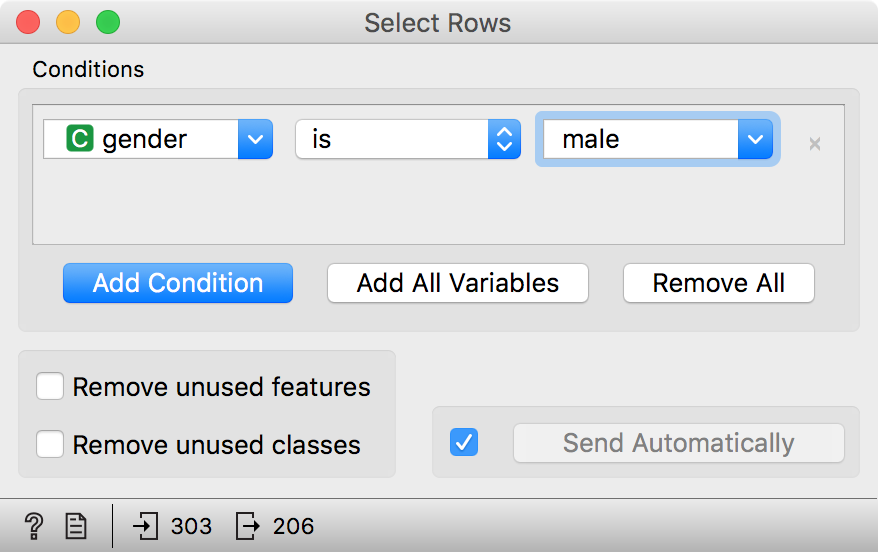
\includegraphics[scale=0.4]{select-rows.png}}
  \newcommand{\distrib}{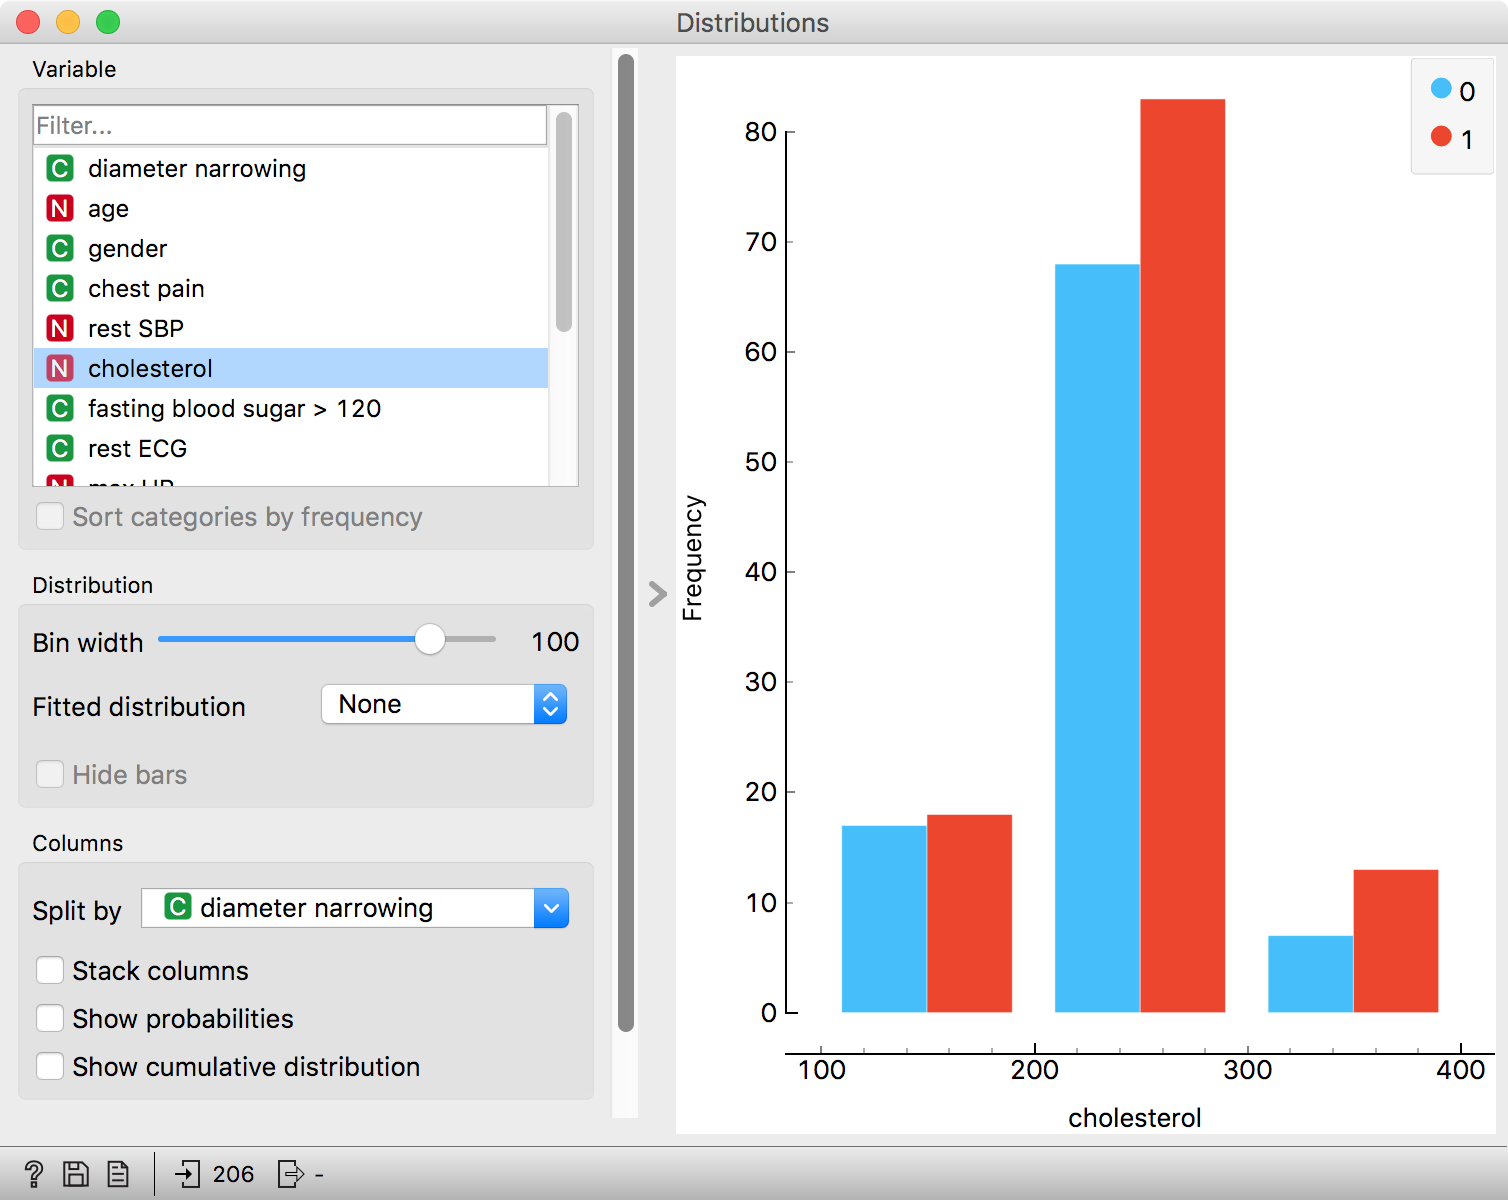
\includegraphics[scale=0.4]{distributions.png}}
  \infinitewidthbox{
  \stackinset{r}{-0.55\linewidth}{t}{+0.1\linewidth}{\distrib}{\selrow}\hspace{8cm}
  }
\end{figure*}

There are two less-known — but great — visualizations for observing interactions between features. 

The mosaic display shows a rectangle split into columns with widths reflecting the prevalence of different types of chest pain. Each column is then further split vertically according to gender distributions within the column. The resulting rectangles are split again horizontally according to age group sizes. The red and blue areas represent each group's outcome distribution within the resulting bars, and the tiny strip to the left of each shows the overall distribution.

\newpage
What can you read from this diagram?

\begin{figure}[h]
  \centering
  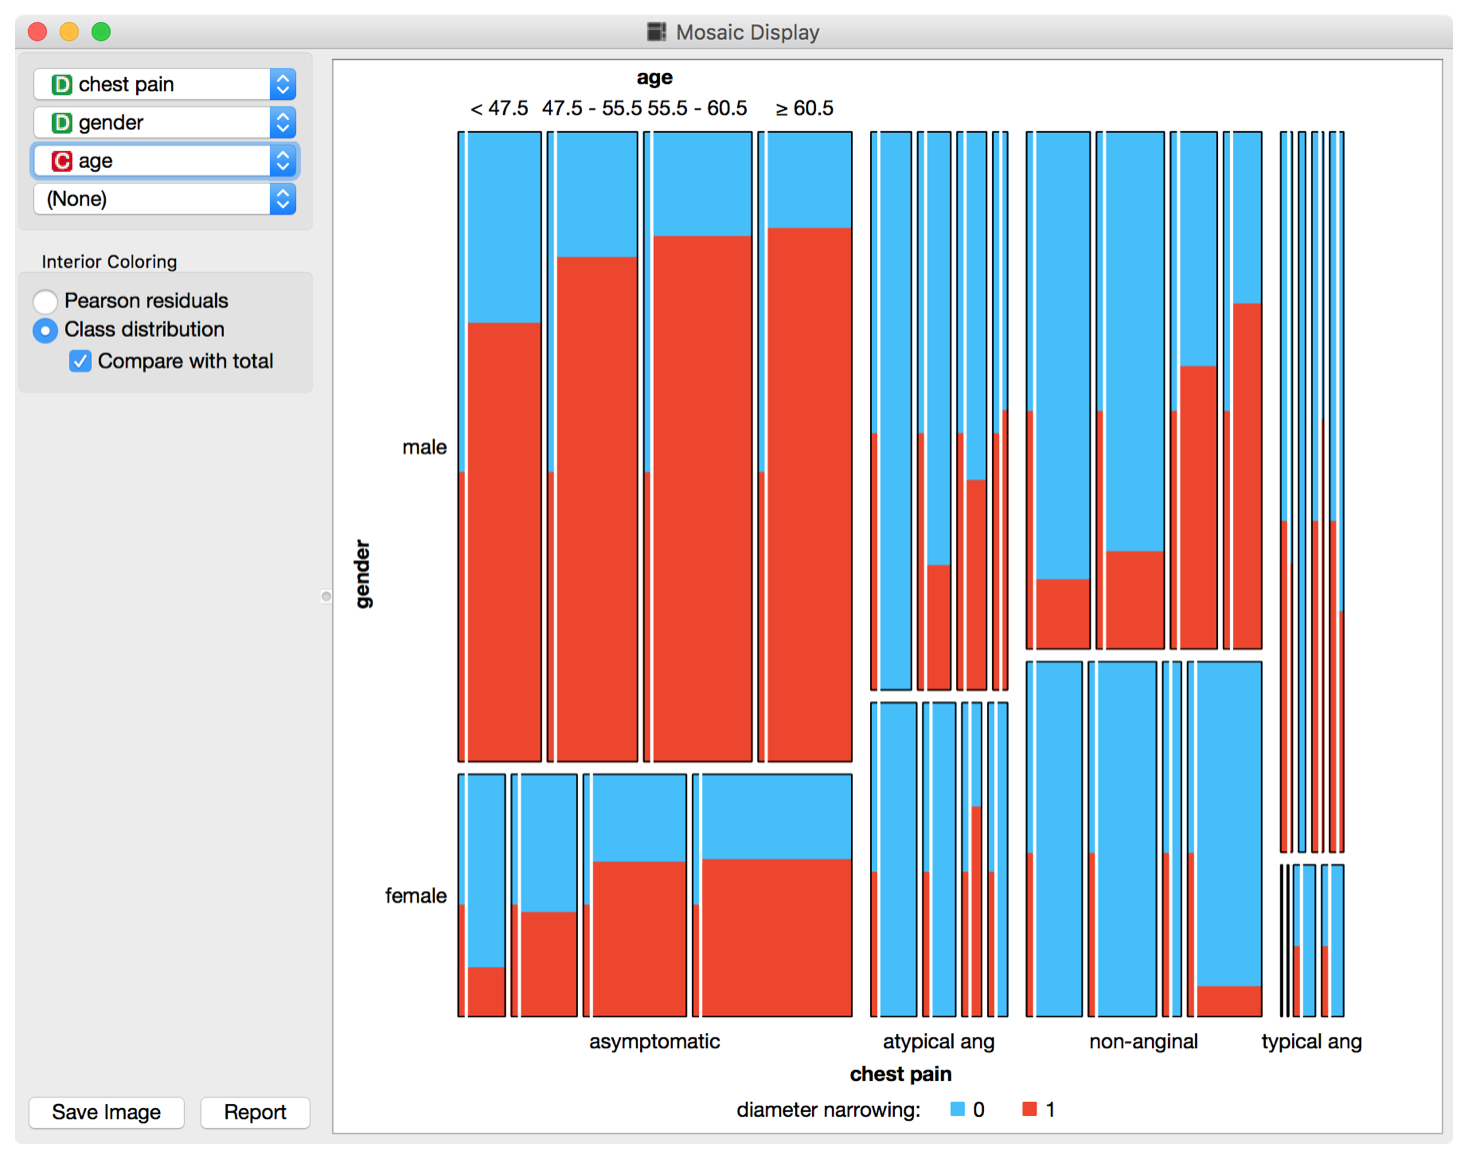
\includegraphics[width=\linewidth]{basic_data_exploration-fig6.png}
  \caption{\textbf{\textsf{You can play with the widget by trying different combinations of 1-4 features.}}}
  \label{fig:basic_data_exploration-fig6}
\end{figure}

\begin{wrapfigure}{o}{0.9\textwidth}
  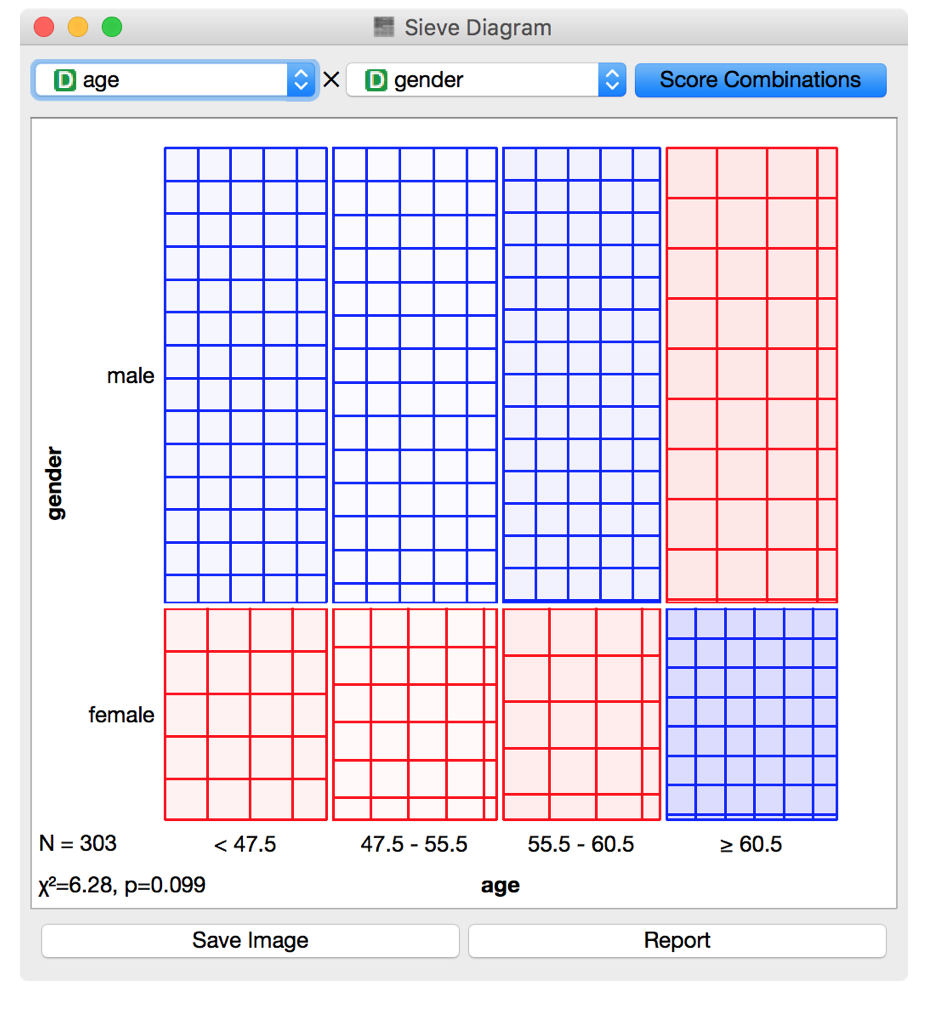
\includegraphics[scale=0.6]{basic_data_exploration-fig7.png}
  \caption{\textbf{\textsf{See the Score Combinations button? Try to guess what it does? And how does it score the combinations? Hint: there are some Greek letters at the bottom of the widget.}}}
\end{wrapfigure}

Another visualization, the Sieve diagram also splits a rectangle horizontally and vertically, but with independent cuts, so the areas correspond to the expected number of data instances if the observed variables were independent. For instance, 1/4 of patients are older than 60, and 1/3 of patients are female, so the area of the bottom right rectangle is 1/12 of the total area. With roughly 300 patients, we would expect $1/12 \times 300 = 25$ older women in our data. Instead, there are 34. The sieve diagram shows the difference between the expected and the observed frequencies by the grid density and the color of the field.
